\documentclass[11pt]{article}

\usepackage[letterpaper, margin=0.75in]{geometry}
\usepackage[utf8]{inputenc}
\usepackage[T1]{fontenc}
\usepackage{graphicx}
\usepackage[french]{babel}

\title{Travail pratique \#2 - IFT-2245}
\author{Maude Sabourin et Jérémy Coulombe} 
\begin{document}

\maketitle
\section{Expérience}
Ce travail a été excessivement frustrant, mettant à l’épreuve notre bien-être mental et physique. Nous avons passé énormément de temps à essayer de comprendre des concepts pourtant simples, et encore plus de temps à essayer de les mettre en pratique de façon fonctionnelle. De nombreuses erreurs, pour la plupart cachée dans les décombres de notre code, ont rendu le travail vraiment lourd et difficile. Sans arrêt, nous devions chercher une aiguille dans une botte de foin. Je crois que nous pouvons sans regret dire que c’est notre pire expérience académique à vie. Cependant, c’est probablement aussi le TP où nous avons appris le plus de choses.

\section{Problèmes rencontrés}
Nous avons rencontré plusieurs problèmes durant ce travail. Tout d’abord, le simple fait de connecter le client et le serveur ensemble nous a pris 2 semaines. Nous ne comprenions rien aux arguments que nous devions envoyer (un port?) et même si nous avions la majorité du code dans server\_thread, nous ne savions même pas si nous pouvions le réutiliser. 

Notre gros problème provenait du getline. Nous ne savions pas qu’il allouait la mémoire (nous ne l’avions pas utilisé au TP1), donc nous faisions 2 malloc. Ensuite, nous avions des segfault à ne plus finir pour des raisons douteuses. Suite à notre incapacité à trouver la raison, nous avons dû recoder l'ensemble du serveur. Cependant, plus tard, nous avons eu un getline qui nous retournait -1 alors que le buffer avait une valeur! Cela ne fait aucun sens! Cette commande a engendré un nombre inimaginable de segfault et nous espérons ne jamais avoir à la réutiliser. Soit elle est carrément boguée (elle ne fonctionne même pas sur cygwin..), soit il faut être un pro pour bien l’utiliser.

Ensuite, notre mauvaise compréhension des concepts clés de la communication nous a encore une fois mis des bâtons dans les roues. Qu’est-ce qu’un socket, qu’un stream, qu’un file descriptor? Quelle est la relation entre ces éléments et comment les utiliser ensemble? Quelle est la différence entre send/receive et write/read et fdopen/fclose? Ce fut beaucoup de notions à assimiler et malheureusement nous les avons malcompris pendant longtemps. Nous pensions que nous avions besoin des trois pour que notre serveur et notre client puissent communiquer. Nous ne comprenions pas aussi Fflush, ce qui a fait que souvent nous écrivions dans le stream (ou dans printf..) et nous ne comprenions pas pourquoi rien ne s’envoyait ou ne s’affichait.

Parlant de printf, nous avons appris l’importance du \textbackslash n  dans l’envoi et la réception des requêtes. De même, le fameux \begin{verbatim} (\0) \end{verbatim} nous a également causé quelques problèmes avec Valgrind. Nous pensions qu’il était équivalent à définir un char* = NULL, mais en fait pas du tout! 

Un autre problème vraiment frustrant a été l’utilisation de Dyn\_array.c. Nous avions modifié le code pour avoir plusieurs versions (une avec un char**, l’autre avec une struct Client que nous avions créé). Cependant, nous n’arrivions pas à bien importer le code sans qu’il y ait un million d’erreurs. Nous avons aussi essayé de l’importer dans le header et il y avait constamment des problèmes avec une double définition des méthodes (puisque main appelle header aussi). Bref, si ce n’était pas assez, nous avons eu beaucoup de problèmes de mémoire, de segfault et via le free. Nous avons évidemment compris qu’utiliser une librairie n’est pas aussi simple qu’il le paraît. Il faut vraiment bien comprendre le code dedans, sinon on peut avoir des surprises. Finalement, nous avons pris l’option de fournir le nombre de clients, car nous étions face à trop de problèmes liées à l’usage d’un array dynamique. Nous avons tout de même gardé la librairie pour le parsing des requêtes\/réponses.

Le pire de tous les problèmes était sans nul doute la recherche des erreurs. Nous avons dû composer avec des problèmes qui n'apparaissaient pas systématiquement. Cela rendait l'identification de la cause exacte difficile. En effet, nous pouvions rouler notre code dix fois et n’avoir que le problème une fois. Il fallait donc espérer retomber dessus pour essayer de le régler. Dans certains cas, nous pouvions procéder par élimination en appliquant des solutions trouvées en ligne (relatives à un message d’erreur reçu) ou encore en essayant de trouver les endroits d’où pourrait provenir le problème. Bien que Valgrind et GDB étaient d'une aide précieuse, ils étaient parfois trop vagues, nous indiquant un segfault (par exemple pour l’envoi de la REQ 1 2 3 …), sans pour autant nous aider à comprendre pourquoi cette requête en particulier boguait. 

Nous avons aussi eu droit à des omissions du compilateur. Par exemple, nous avions déclaré deux fois plusieurs mutex et nous n'avons eu aucun warning et aucune erreur. Nous avions aussi une connexion avec le serveur sur laquelle il n'y avait aucune information qui était envoyée ce qui causait un segfault. Il y a certaines erreurs dont nous n'avons jamais trouvé l'origine et ce n'est pas faute d'avoir essayé. Cependant, notre code roule bien dans la majorité des cas, ce qui est en soi une grosse victoire. 

Quelques autres difficultés sont par exemple le CLO, qui ne retournait pas au main, ou le end qui avait un comportement étrange (segfault et erreurs). Les compteurs étaient aussi incrémentés au mauvais endroit, car nous ne comprenions pas bien la définition de chacun dans le code. Nous avions essayé de créer une fonction pour incrémenter les compteurs sans penser qu’il fallait passer la référence au pointeur, sinon c’était la variable locale qui était incrémentée!

Finalement, le top 3 des erreurs les plus fréquentes a été
1) Segfault : Surtout dû au fclose et au free des tableaux

2) Double Free : Puisque notre code se promène d’une fonction à l’autre, il était parfois difficile de suivre qui avait été free et qui ne l’avait pas été. Nous avons donc rajouté beaucoup de if(...) free(...) pour contrer cela.

3) Too many open files : Segfault déguisé


\section{Ce qui a bien été (oui, il y en a!)}

Parsing : Nous avions déjà une bonne base avec le TP1 donc le parsing de la commande en un array a fonctionné dès le début et n’a jamais causé de problème. Youhou!

Free : Maintenant que nous savions que nous devions free les mallocs, nous avons eu beaucoup moins de difficulté à le faire. Nous avons eu quelques problèmes de double free, mais au moins, nos fuites de mémoire étaient presque inexistantes.

Strcmp vs Strstr : Nous avons eu quelques problèmes avec le caractère final (\begin{verbatim} \0 \end{verbatim}) et la reconnaissance du pattern envoyé (\textbackslash n), mais en général, nous avions utilisé ces fonctions dans le TP1 et ça a paru!

Valgrind : Relativement au free, nous n’avions presque aucune fuite mémoire. Nous avons ajouté -v pour avoir les détails et avons rapidement su où aller et quoi faire, grâce au TP1. Nous avons porté une attention particulière à la gestion mémoire après avoir perdu des points lors du TP1 sur cet aspect. Nous sommes super fiers de dire que pour client et pour serveur, nous n’avons aucune fuite mémoire! 

PHOTO ICI

Lock : Nous avons implémenté les lock des variables globales dès le début de notre application. Nous n’avons ainsi jamais eu de problème de condition de course.

Protection input : Nous avions perdu des points au TP1, car nous ne gérions pas les mauvais inputs usager. Nous nous sommes repris cette fois-ci. L’usager ne peut entrer des nombres négatifs ou des lettres lors que l’initialisation du programme. 
\section{Décisions prises}
Connexion répétée : Nous avons décidé que le client devrait établir une connexion avec le serveur à chaque fois qu'il veut envoyer une commande et il fermerait cette connexion après avoir reçu une réponse du serveur. Cette décision a amené son lot de difficulté, car cela occasionnait une gestion des connexions beaucoup plus minutieuse. La raison est simple : le serveur (représentant un genre de thread noyau), ne devrait pas avoir à attendre après le client. Cette architecture nous permet de faire WAIT un client et d’accepter les requêtes du prochain. C’est donc beaucoup plus optimal, même si ça a été un gros défi d’en réussir l’implémentation. 

Getline : Nous avions d’abord pensé utiliser la fonction getdelim, mais un de nos démonstrateurs nous a  montré les problèmes que cette fonction pourrait causer. Nous nous sommes donc tournés vers getline, qui franchement n’a pas été plus simple, mais qui, nous l’espérons, causera moins de problèmes (dans Valgrind, nous avons vu que getline appelle getdelim! Toute une surprise!).

Gestion input client : Au début, le serveur faisait une vérification exhaustive des entrées du client. Cependant, nous avons décidé d’envoyer cette gestion au client directement puisque c’est lui qui gère l’input de l’usager.

FdOpen : Après réflexion, il aurait probablement été mieux d’utiliser send/receive avec des buffers et memset. La raison est que nous avions énormément de problèmes avec les fclose qui faisaient des segfault à d’autres endroits.

Multithreading : Lors de l’implémentation de la fonction de parsing de la commande, nous avions initialement utilisé strtok. Or, cette fonction n'est pas réentrante donc elle n'est pas sécuritaire pour le multithreading. Nous avons donc dû utiliser une de ses variantes dont nous avons découvert l'existence sur stackOverflow (strtok\_r). Cet exemple reflète bien l'ensemble du tp puisqu'il nécessitait un grand effort de recherche afin de comprendre les méthodes nécessaires, les messages d'erreurs et autres composantes du TP.

Array Dynamique : Tel que mentionné un peu plus tôt, nous avons fait de notre mieux pour implémenter cette fonctionnalité, mais cela causait vraiment beaucoup de problèmes. Nous avons conservé un seul array dynamique dans lequel nous stockons chacun des mots de la commande reçue par le serveur ou de la réponse que le client reçoit du serveur.
 
\section{Faiblesses \& Améliorations possibles}
Wait : environ 1 fois sur 10, notre banquier reste pris dans une loop où il fait WAIT tous les clients. Nous avons investigué longuement sur ce problème et nous n’avons jamais compris la cause. L’algorithme est conforme à celui vu en classe et les requêtes sont ont le bon nombre de demandes. Deux causes sont possibles :
- Soit le serveur ‘saute’ une requête, parfois dû à un envoi bogué dans le socket (où le serveur envoie du vide au client)
- Soit il accepte une requête avant d’avoir les autres (style il accepte une REQ avant d’avoir tous les INI), donc il alloue les ressources et ensuite se rend compte qu’il est bloqué.

Dans les récents tests que nous avons faits, nous n’avons pas réussi à reproduire ce bogue. Cependant, il est possible qu’il refasse surface lors de vos tests.


\section{Fonctionnement de notre code}

PHOTOS ICI
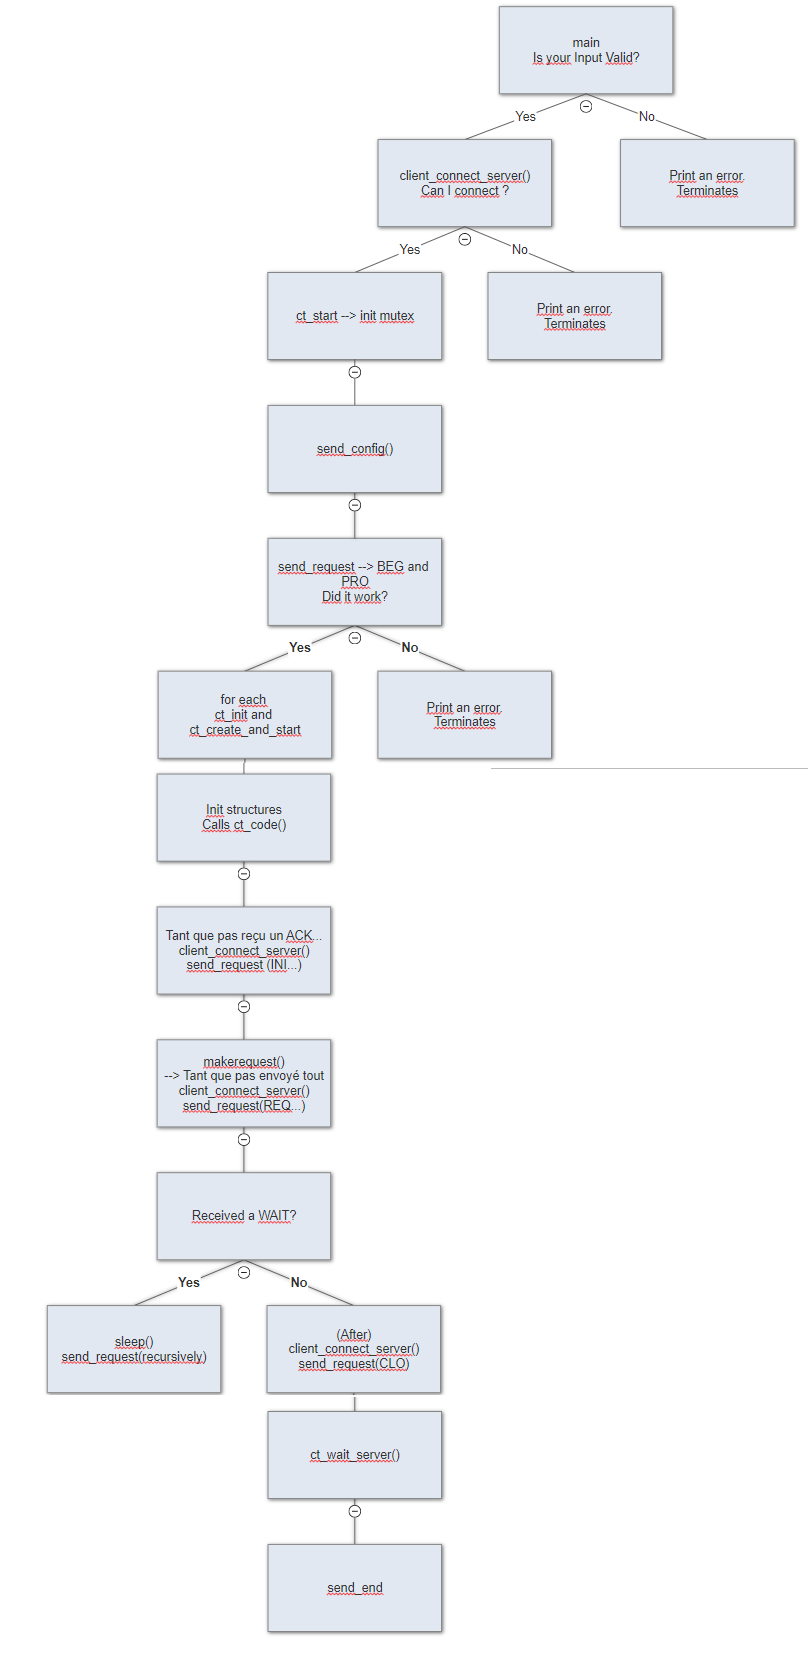
\includegraphics[width=\textwidth,height=\textheight,keepaspectratio]{CLIENT}

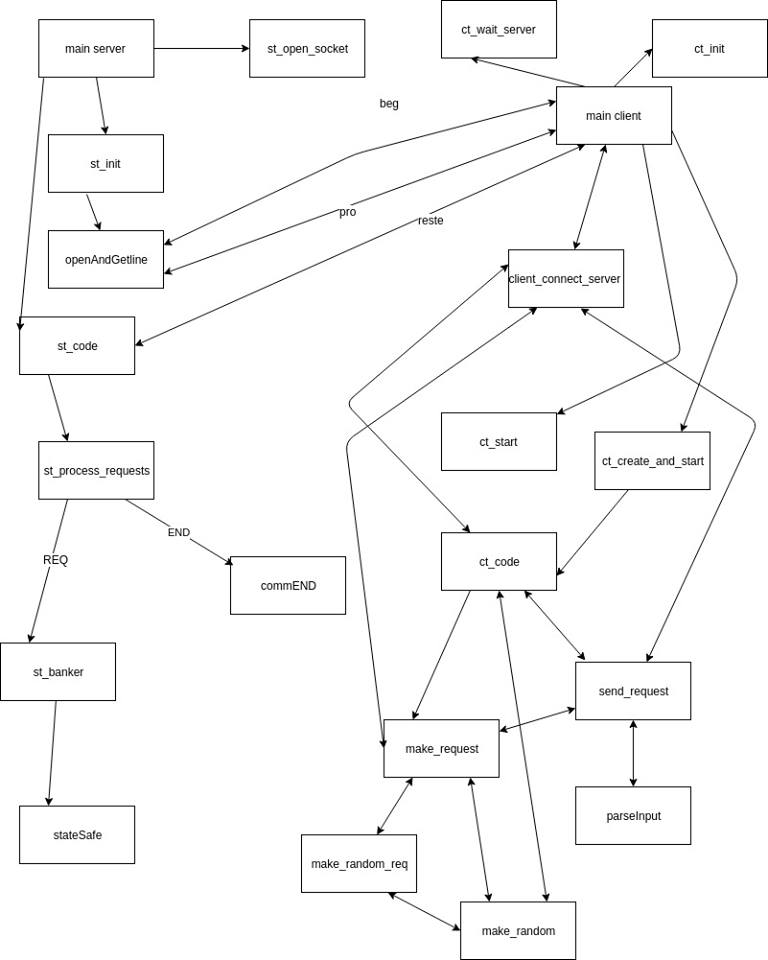
\includegraphics[width=\textwidth,height=\textheight,keepaspectratio]{CLIENTEtSERVER}





%% ¡¡ REMPLIR ICI !!

\end{document}
